\documentclass[brazilian, fleqn]{article}

\usepackage{babel}
\usepackage[utf8]{inputenc}
\usepackage[T1]{fontenc}
\usepackage{lmodern}

\usepackage{amssymb,amsfonts,amsmath}

\usepackage{tikz}
\usetikzlibrary{calc}

\usepackage[left=2cm, bottom=2cm, right=1.5cm, top=1.5cm]{geometry}

\usepackage{siunitx}
\sisetup{locale = FR}

\usepackage{tcolorbox}
\tcbuselibrary{skins}
\tcbset{boxrule=0pt, top=0pt, bottom=0pt, skin=bicolor, interior style={left color=black!10}}

\DeclareMathOperator{\sen}{sen}
\DeclareMathOperator{\tg}{tg}

\begin{document}
\section*{\centering Questão de aluno 15/04/2023}

\begin{center}
    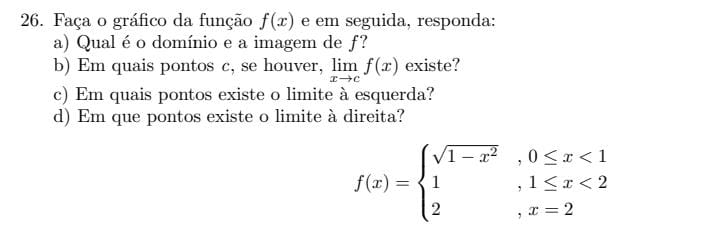
\includegraphics[width=\textwidth]{quest-2.jpg}
\end{center}

\textit{Solução}:\\
\begin{center}
    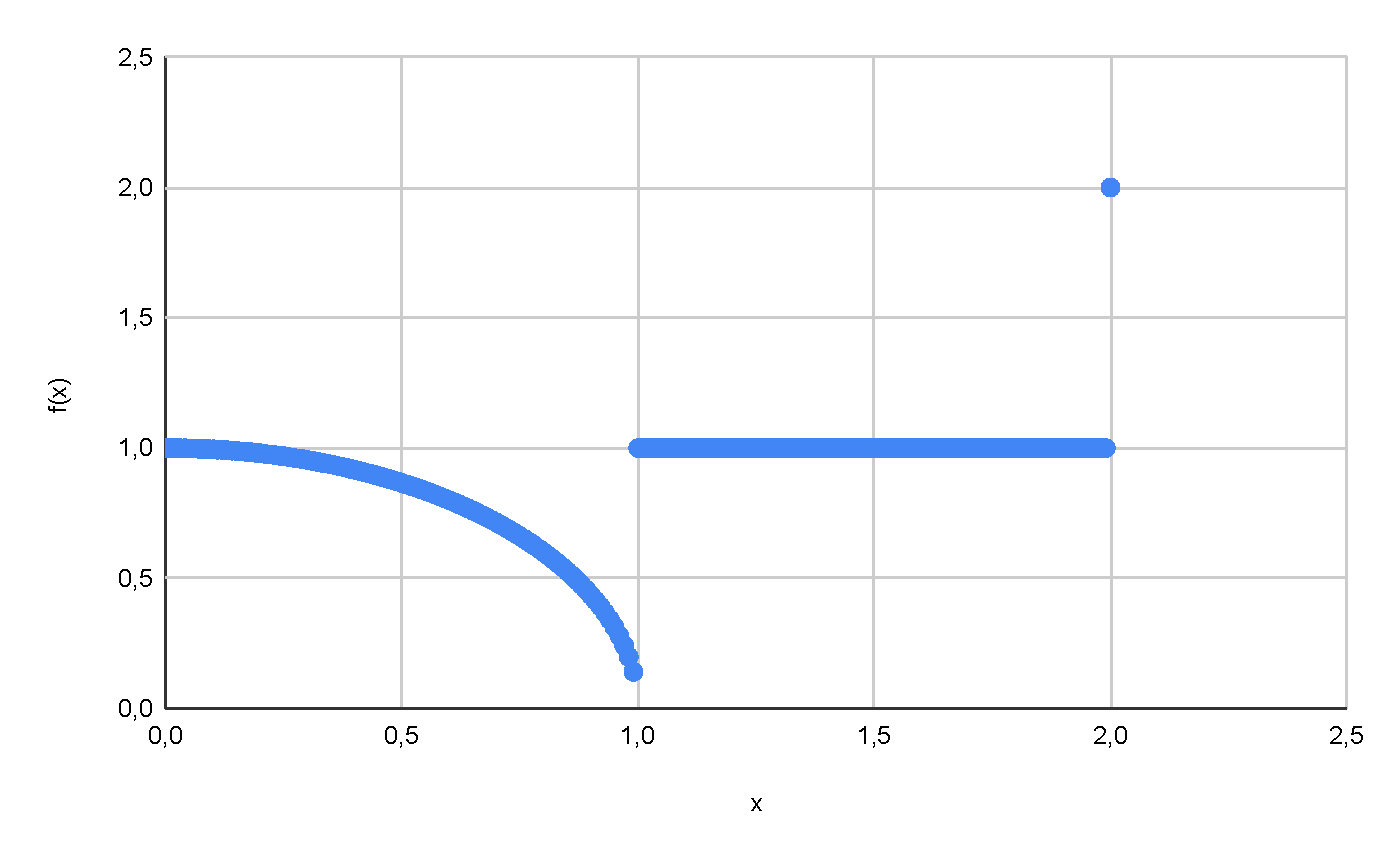
\includegraphics[width=\textwidth]{chart (1).pdf}
\end{center}

a) \(\text{domínio} = \{0 \leq x \leq 2\}\), 
\(\text{imagem}=\{0 < f(x) \leq 1\} \cup \{x=2\}\)

b) \(0 < x < 1\) e \(1 < x < 2\)

c) \(0 < x \leq 1\) e \(1 < x \leq 2\)

d) \(0 \leq x < 1\) e \(1 \leq x < 2\)
\end{document}
